% planisphere.tex
%
% The LaTeX code in this file brings together into a single document the
% various components of the model planisphere.
%
% Copyright (C) 2014-2019 Dominic Ford <dcf21-www@dcford.org.uk>
%
% This code is free software; you can redistribute it and/or modify it under
% the terms of the GNU General Public License as published by the Free Software
% Foundation; either version 2 of the License, or (at your option) any later
% version.
%
% You should have received a copy of the GNU General Public License along with
% this file; if not, write to the Free Software Foundation, Inc., 51 Franklin
% Street, Fifth Floor, Boston, MA  02110-1301, USA

% ----------------------------------------------------------------------------


\documentclass[a4paper, portrait, margin = 2.2em]{article}
\usepackage[dvips]{graphicx}
\usepackage{fancyhdr,url}
\usepackage[utf8]{inputenc}
\usepackage[pdftitle={Crie seu próprio planisfério}, pdfauthor={Arthur Rosso}, pdfsubject={Crie seu próprio planisfério}, pdfkeywords={Crie seu próprio planisfério}, colorlinks=true, linkcolor=blue, citecolor=blue, filecolor=blue, urlcolor=blue]{hyperref}
\usepackage[T1]{fontenc}
\usepackage{xcolor}
\pagecolor{black}
\color{white}

\title{Faça seu próprio planisfério}
\author{Arthur Rosso}
\date{2019}

\begin{document}
\thispagestyle{empty}
\begin{center}
\begin{tabular}{ | c | } 
    \hline
    \centerline{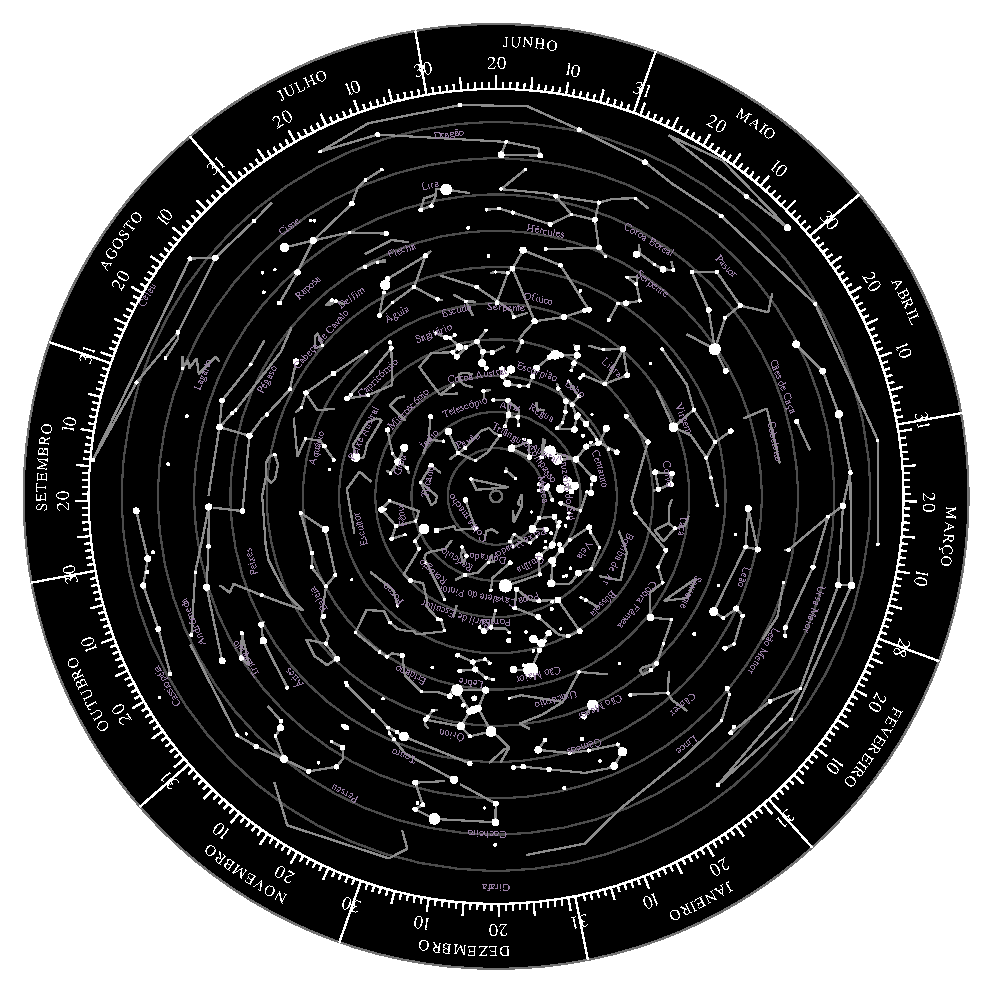
\includegraphics{tmp/starwheel}}

    \centerline{I love you to the moon and back.}
    
\end{tabular}
\end{center}

\begin{center}
    \begin{tabular}{||c c c c||} 
    \hline
    Col1 & Col2 & Col2 & Col3 \\ [0.5ex] 
    \hline\hline
    1 & 6 & 87837 & 787 \\ 
    \hline
    2 & 7 & 78 & 5415 \\
    \hline
    3 & 545 & 778 & 7507 \\
    \hline
    4 & 545 & 18744 & 7560 \\
    \hline
    5 & 88 & 788 & 6344 \\ [1ex] 
    \hline
   \end{tabular}
   \end{center}

\end{document}

